% Introduction - A bit description of Blockchain and the problem statement you are working on
% Chapter Template

\chapter{Introduction} % Main chapter title

\label{Chapter 1} % Change X to a consecutive number; for referencing this chapter elsewhere, use \ref{ChapterX}

\lhead{Chapter 1. \emph{Introduction}} % Change X to a consecutive number; this is for the header on each page - perhaps a shortened title

%----------------------------------------------------------------------------------------
%	SECTION 1
%----------------------------------------------------------------------------------------
\section{What is a blockchain?}



A blockchain is a growing list of records, called blocks, which are linked using cryptography. Each block contains a cryptographic hash of the previous block, a timestamp, and transaction data (generally represented as a merkle tree root hash).

By design, a blockchain is resistant to modification of the data. It is "an open, distributed ledger that can record transactions between two parties efficiently and in a verifiable and permanent way". For use as a distributed ledger, a blockchain is typically managed by a peer-to-peer network collectively adhering to a protocol for inter-node communication and validating new blocks. Once recorded, the data in any given block cannot be altered retroactively without alteration of all subsequent blocks, which requires consensus of the network majority. Although blockchain records are not unalterable, blockchains may be considered secure by design and exemplify a distributed computing system with high Byzantine fault tolerance. Decentralized consensus has therefore been claimed with a blockchain.

\section{Problem Statement}

A blockchain system's throughput depends on the number of nodes participating in the validation of a transaction. More the number of nodes means more resistance to faults but resulting in higher latency and lower throughputs. The objective of this project is to propose a blockchain system where the number of validators is determined by the market dynamics.


% \paragraph{Literature Survey}

% This is a sample. Write about referred papers. Cite like this \citep{nip2010cyclic}. Another example would be this \citep{nip2010extremely}. More citations like this \citep{bird2004evaluating}, \citep {tremblay2003seismic} and \citep {alhamaydeh2016key}.

% \paragraph{Research gaps}
% Typically include research gaps for your study. 
% \paragraph{Objective}
% Similarly objectives of study. 
% \paragraph{Scope}
% Define scope of study. 
% \paragraph{An algorithm}
% How you could refer to figures: This is an example. (Refer \ref{fig5}). You can add equations like this Eq. (\ref{eq1})
% \begin{equation}
% \label{eq1}
%   SDR = sd(T) - \sum_{i}\frac{{T}_{i}}{|T|}\times sd({T}_{i})
% \end{equation}

% \begin{figure}[]
% \centering
% 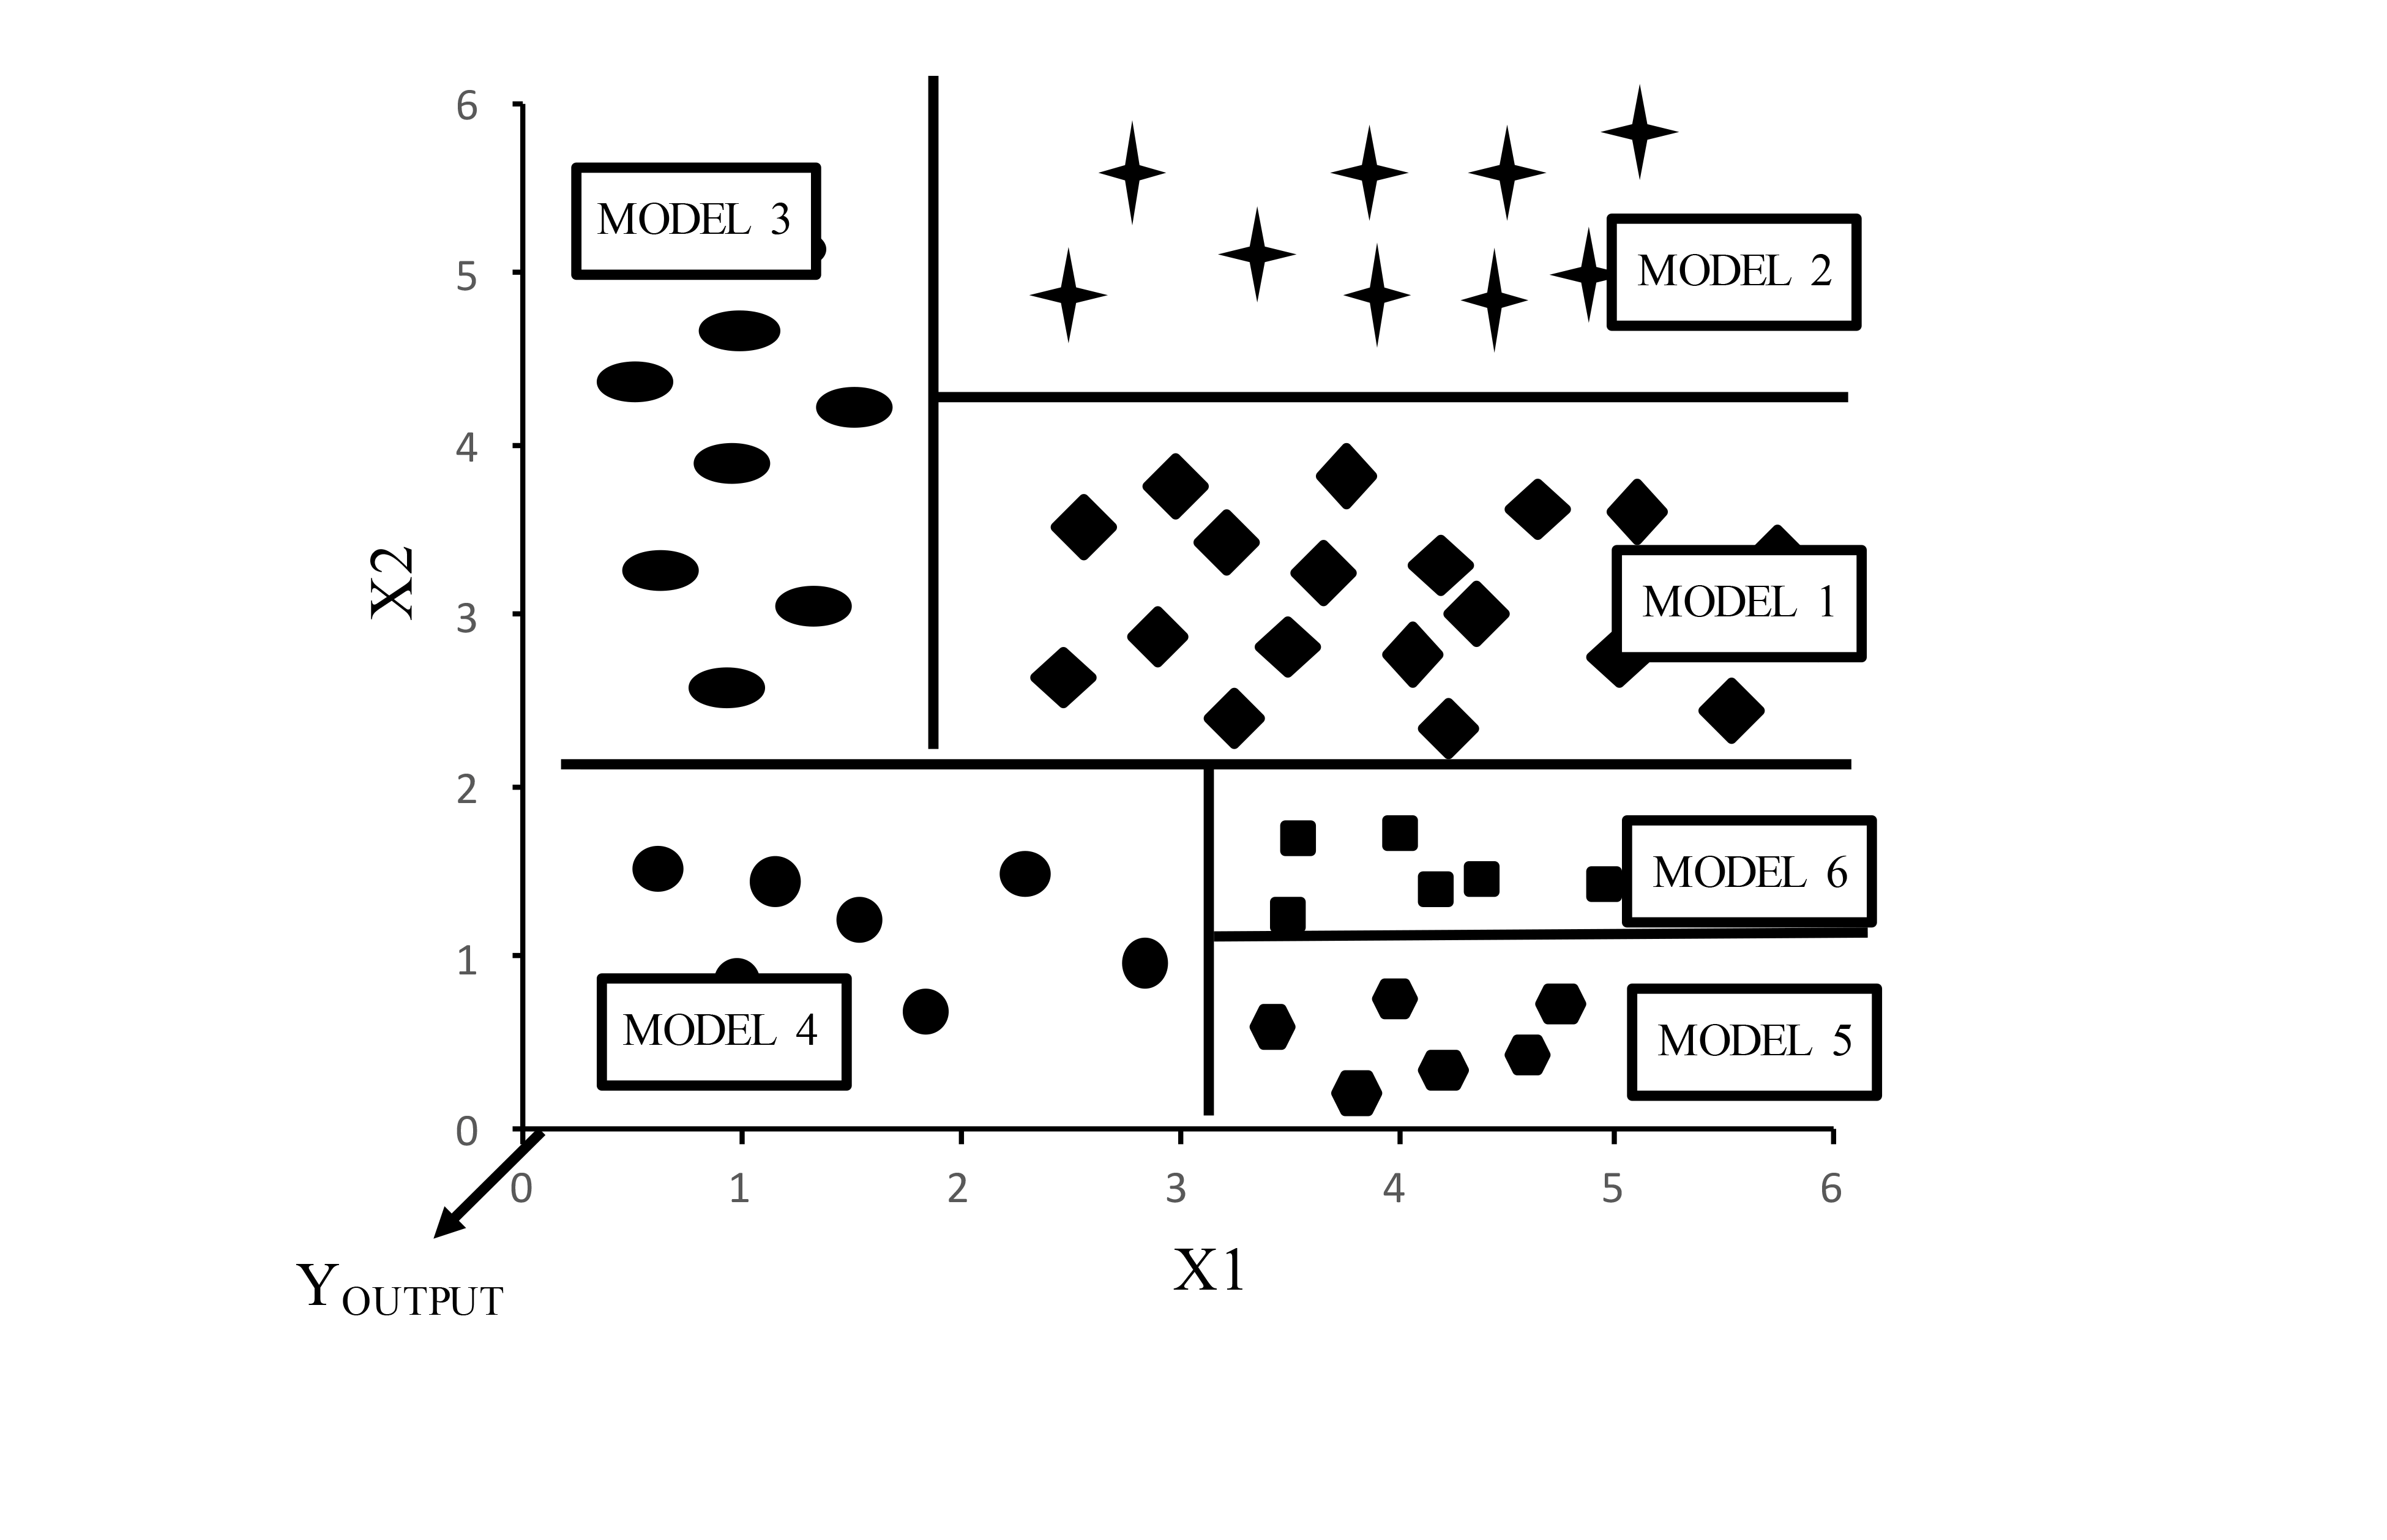
\includegraphics[height=7cm]{splits.png}
% \caption{Splitting of the input space (X1 x X2) by M5' model tree algorithm}
% \label{fig5}
% \end{figure}

% \section{Adding another section}
% You can show a lot of figures together like these Figures \ref{fig61}, \ref{fig62}, \ref{fig63} below.
% \begin{figure} [!htbp]
% \centering    
% \subfigure[Caption1]{\label{fig61}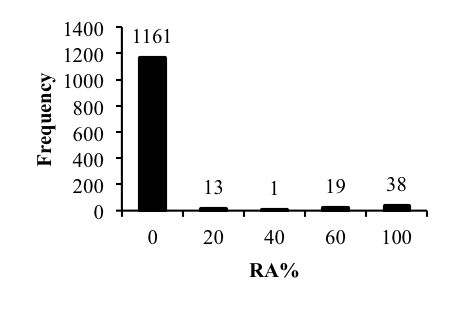
\includegraphics[width=42mm]{data1.png}}
% \subfigure[Caption2]{\label{fig62}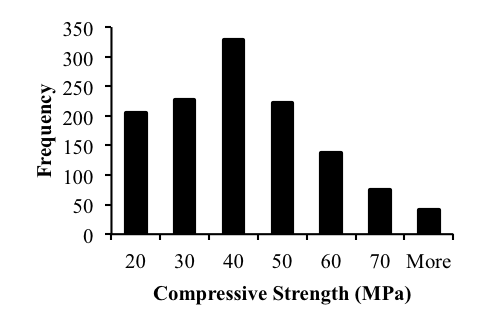
\includegraphics[width=42mm]{data2.png}}
% \subfigure[Caption3]{\label{fig63}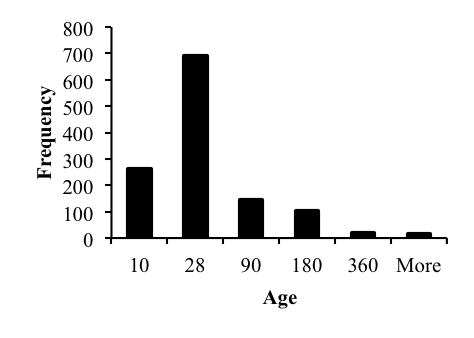
\includegraphics[width=42mm]{data3.png}}
% \caption{Figures sample}
% \end{figure}
% You can add lists into the text like this. 
% \begin{itemize}
% \settowidth{\leftmargin}{{\Large$\square$}}\advance\leftmargin\labelsep
% \itemsep3pt\relax
% \renewcommand\labelitemi{{\lower1pt\hbox{\small$\square$}}}
% \item	Some sample text item 1. 
% \item You may refer to tables \ref{tab1} 
% \item Or figures \ref{fig61}
% \end{itemize}

% Tables can be added like this
% \begin{table}[!htbp]
% \centering
% \caption{Sample table}
% \label{tab1}
% \begin{tabular}{llll}

% \hline
% Column 1 & Column 2 & Column 3       \\\hline
% 1         & Data1 & 13.41179 & 0.9492839 \\
% 2            & Data2 & 13.39824 & 0.9492952\\\hline
% \end{tabular}
% \end{table}


